
\chapter{Systematic Uncertainties}
\label{chap:Uncertainties}

\indent Systematic uncertainties can be separated into two separate categories, experimental uncertainties and theoretical uncertainties.  Experimental systematics result from uncertainties in physics object reconstruction, calibration, the understanding of the detectors and the amount of additional pileup interactions.  Theoretical systematics result from uncertainties in PDFs, interaction scales, and theoretical calculations. Experimental uncertainties such as jet energy resolution are assumed to be 100 percent correlated across different background sources.  On the other hand, theoretical uncertainties are assumed to be uncorrelated from one another.  \\

\indent In general systematic uncertainties are parameterized as independent parameters with gaussian constraints.  These parameters are called ``nuisance'' parameters and normally denoted by the symbol $\alpha$.  The systematic errors on backgrounds are evaluated through a simultaneous fit to the CR and the SR.  An estimate of the systematic uncertainties on backgrounds in the SR can be made by fitting to the CR alone and extrapolating the result to the SR.  It is important to note that the fit can also lead to correlations between initially independent systematics uncertainties. \\

\indent The amount of MC background in both the CR and SR will vary with experimental and theoretical systematics before the fit.  However after the fit the total amount of background will be normalized to the CR.  If the MC yield for background has a downward variation for a given systematic then the normalization scale factor will increase.  The increased normalization scale factor will compensate for the simultaneous drop in SR MC yield.  This partial cancelation of fluctuations between CR and SR can lead to smaller systematic uncertainties.  In effect, the CR reduces systematic uncertainty by directly measuring the amount of background in from data instead of relying solely on MC simulations.\\

%If the background prediction varies in the same way in the CR and the SR the total systematic in SR is partially canceled out in the transfer factor.  

\indent This is why designing a CR that is kinematically similar to the SR is crucial to mitigating systematic uncertainties.  More detail on CR design and systematics can be found in chapter \ref{sec:Bkg:Tech} on background estimation and chapter \ref{chap:statistics} on statistics analysis.  \\

%\indent The fit may compensate for a change in one systematic by varying several other systematics in order to get the best fit in CR.  The correlation matrix between a reduced set of systematic variations and background scale factor after the simultaneous fit to all CRs are given in figure \ref{figure.corrMatrix}.

%\indent The fit can also lead to correlations between systematics that are initially parameterized as independent nuisance parameters before the fit to CR.    The scale factor $\mu$ is the amount that the expected background MC must be scaled up/down by so that data and MC yields agree in the CR.  \\

\indent The total background systematic uncertainty is $\approx 20\%$ in the SR.  The dominant background systematic uncertainties in the first four $\RISR$ SR bins, between $0.3 < \RISR < 0.7$, include uncertainty on the ttbar ISR/FSR, and uncertainty on the ttbar matrix element and parton shower calculation and uncertainty on the jet energy resolution.  Each of these dominant systematic uncertainties contributes 5-10\% to the total uncertainty on background rate in the SR.  The theoretical uncertainty on the amount of interference between SM ttbar and single top at NLO is also significant.  \\

\indent The large systematic uncertainty in the highest $\RISR$ bin between $0.7-0.8$ is completely due to low MC statistics caused by the low expected yield.  However the $0.7-0.8$ $\RISR$ region is completely statistically dominated for the same reason, with only 0.7 expected background events.  \\

\indent The dominant background uncertainties in each SR bin is given in table \ref{table.results.bkgestimate.uncertainties.SRC1_SRC2_SRC3} and \ref{table.results.bkgestimate.uncertainties.SRC4_SRC5}.  \\

%\begin{table}[htpb]
  %\caption{5 Largest Systematic Uncertainty on SM background in the Signal Region. }
  % \label{tab:sys:summary}
 % \begin{center}
 %   \def\arraystretch{1.4}%
 %   \begin{tabular}{c|c|c|c|c|c} \hline\hline
%      {\bf $\RISR$ region} &  0.3-0.4 & 0.4-0.5 & 0.5-0.6 & 0.6-0.7 & 0.7-0.8  \\ \hline 
%    \end{tabular}
 % \end{center}
%\end{table}%


\begin{table}
\caption[Breakdown of statistical and systematic uncertainty on background estimates]{
Breakdown of the dominant systematic uncertainties on background estimates.
Note that the individual uncertainties can be correlated, and do not necessarily add up quadratically to 
the total background uncertainty. The percentages show the size of the uncertainty relative to the total expected background.
\label{table.results.bkgestimate.uncertainties.SRC1_SRC2_SRC3}}
\begin{center}
\setlength{\tabcolsep}{0.0pc}
\begin{tabular*}{\textwidth}{@{\extracolsep{\fill}}lccc}
\noalign{\smallskip}\hline\noalign{\smallskip}
{\bf Uncertainty of channel}                                    & SRC1            & SRC2            & SRC3            \\
\noalign{\smallskip}\hline\noalign{\smallskip}
%%
Total background expectation             &  $20.56$        &  $27.54$        &  $18.86$       \\
%% \\
\noalign{\smallskip}\hline\noalign{\smallskip}
%%
Total statistical $(\sqrt{N_{\rm exp}})$              & $\pm 4.53$        & $\pm 5.25$        & $\pm 4.34$       \\
%%
Total background systematic               & $\pm 6.62\ [32.18\%] $        & $\pm 4.89\ [17.75\%] $        & $\pm 3.53\ [18.72\%] $             \\
\noalign{\smallskip}\hline\noalign{\smallskip}
\noalign{\smallskip}\hline\noalign{\smallskip}
%%
ttbar ME/PS uncertainty         & $\pm 4.86\ [23.6\%] $          & $\pm 1.91\ [6.9\%] $          & $\pm 2.39\ [12.7\%] $       \\
%%
ISR/FSR uncertainty                                & $\pm 2.64\ [12.8\%] $          & $\pm 2.19\ [8.0\%] $          & $\pm 1.06\ [5.6\%] $       \\
%%
Single Top Theory Uncertainty          & $\pm 1.66\ [8.1\%] $          & $\pm 1.18\ [4.3\%] $          & $\pm 1.21\ [6.4\%] $       \\
%%
MC statistics in SR bin        & $\pm 1.29\ [6.3\%] $          & $\pm 1.42\ [5.1\%] $            & $\pm 0.96\ [5.1\%] $       \\
%%
ttbar CR normalization factor         & $\pm 0.91\ [4.4\%] $          & $\pm 1.55\ [5.6\%] $          & $\pm 1.03\ [5.4\%] $       \\
%%
Jet energy resolution         & $\pm 0.81\ [3.9\%] $          & $\pm 2.70\ [9.8\%] $          & $\pm 1.14\ [6.0\%] $       \\
%%
QCD Jet Smearing Uncertainty        & $\pm 2.38\ [11.6\%] $          & $\pm 0.77\ [2.8\%] $          & $\pm 0.17\ [0.91\%] $       \\
%%
%alpha\_JET\_GroupedNP\_3         & $\pm 0.72\ [3.5\%] $          & $\pm 0.03\ [0.10\%] $          & $\pm 0.17\ [0.89\%] $       \\
%%
%mu\_SingleTop         & $\pm 0.56\ [2.7\%] $          & $\pm 0.40\ [1.4\%] $          & $\pm 0.41\ [2.2\%] $       \\
%%
%alpha\_MET\_SoftTrk\_ResoPerp         & $\pm 0.46\ [2.3\%] $          & $\pm 0.56\ [2.0\%] $          & $\pm 0.22\ [1.2\%] $       \\
%%
%alpha\_cEff         & $\pm 0.43\ [2.1\%] $          & $\pm 0.40\ [1.5\%] $          & $\pm 0.11\ [0.60\%] $       \\
%%
%alpha\_JET\_GroupedNP\_2         & $\pm 0.30\ [1.5\%] $          & $\pm 0.78\ [2.8\%] $          & $\pm 0.36\ [1.9\%] $       \\
%%
%alpha\_JET\_GroupedNP\_1         & $\pm 0.27\ [1.3\%] $          & $\pm 0.06\ [0.23\%] $          & $\pm 0.04\ [0.19\%] $       \\
%%
%alpha\_MET\_SoftTrk\_Scale         & $\pm 0.23\ [1.1\%] $          & $\pm 0.29\ [1.0\%] $          & $\pm 0.08\ [0.45\%] $       \\
%%
%alpha\_theoSysDiboson         & $\pm 0.19\ [0.94\%] $          & $\pm 0.10\ [0.37\%] $          & $\pm 0.14\ [0.76\%] $       \\
%%
%alpha\_CExtrap         & $\pm 0.16\ [0.80\%] $          & $\pm 0.31\ [1.1\%] $          & $\pm 0.19\ [1.0\%] $       \\
%%
%alpha\_LightEff         & $\pm 0.15\ [0.74\%] $          & $\pm 0.22\ [0.80\%] $          & $\pm 0.04\ [0.23\%] $       \\
%%
%alpha\_bEff         & $\pm 0.14\ [0.70\%] $          & $\pm 0.00\ [0.01\%] $          & $\pm 0.07\ [0.36\%] $       \\
%%
%alpha\_JET\_EtaNonClosure         & $\pm 0.11\ [0.54\%] $          & $\pm 1.13\ [4.1\%] $          & $\pm 0.01\ [0.03\%] $       \\
%%
%mu\_Wjets         & $\pm 0.09\ [0.45\%] $          & $\pm 0.22\ [0.81\%] $          & $\pm 0.22\ [1.2\%] $       \\
%%
%alpha\_theoSysW         & $\pm 0.09\ [0.45\%] $          & $\pm 0.24\ [0.88\%] $          & $\pm 0.23\ [1.2\%] $       \\
%%
%alpha\_MET\_SoftTrk\_ResoPara         & $\pm 0.07\ [0.35\%] $          & $\pm 0.19\ [0.68\%] $          & $\pm 0.03\ [0.15\%] $       \\
%%
%mu\_TtbarV         & $\pm 0.05\ [0.22\%] $          & $\pm 0.09\ [0.34\%] $          & $\pm 0.09\ [0.47\%] $       \\
%%
%alpha\_PILEUP         & $\pm 0.02\ [0.11\%] $          & $\pm 0.32\ [1.2\%] $          & $\pm 0.12\ [0.64\%] $       \\
%%
%alpha\_FTExtrap         & $\pm 0.02\ [0.11\%] $          & $\pm 0.04\ [0.13\%] $          & $\pm 0.03\ [0.17\%] $       \\
%%
%alpha\_theoSysTTbarV         & $\pm 0.01\ [0.07\%] $          & $\pm 0.03\ [0.11\%] $          & $\pm 0.03\ [0.15\%] $       \\
%%
%alpha\_JVT         & $\pm 0.01\ [0.06\%] $          & $\pm 0.04\ [0.13\%] $          & $\pm 0.04\ [0.22\%] $       \\
%%
%gamma\_stat\_SRC2\_cuts\_bin\_0         & $\pm 0.00\ [0.00\%] $          & $\pm 1.42\ [5.1\%] $          & $\pm 0.00\ [0.00\%] $       \\
%%
%gamma\_stat\_SRC3\_cuts\_bin\_0         & $\pm 0.00\ [0.00\%] $          & $\pm 0.00\ [0.00\%] $          & $\pm 0.96\ [5.1\%] $       \\
%%
\noalign{\smallskip}\hline\noalign{\smallskip}
\end{tabular*}

\begin{tabular*}{\textwidth}{@{\extracolsep{\fill}}lcc}
\noalign{\smallskip}\hline\noalign{\smallskip}
{\bf Uncertainty of channel}                                    & SRC4            & SRC5            \\
\noalign{\smallskip}\hline\noalign{\smallskip}
%%
Total background expectation             &  $7.69$        &  $0.90$       \\
%% \\
\noalign{\smallskip}\hline\noalign{\smallskip}
%%
Total statistical $(\sqrt{N_{\rm exp}})$              & $\pm 2.77$        & $\pm 0.95$       \\
%%
Total background systematic               & $\pm 1.37\ [17.77\%] $        & $\pm 0.71\ [78.68\%] $             \\
\noalign{\smallskip}\hline\noalign{\smallskip}
\noalign{\smallskip}\hline\noalign{\smallskip}
%%
ttbar ME/PS uncertainty        & $\pm 0.68\ [8.8\%] $          & $\pm 0.63\ [69.1\%] $       \\
%%
ISR/FSR uncertainty        & $\pm 0.46\ [6.0\%] $          & $\pm 0.13\ [14.8\%] $       \\
%%
Single Top Theory Uncertainty        & $\pm 0.71\ [9.3\%] $          & $\pm 0.00\ [0.00\%] $       \\
%%
MC statistics in SR bin         & $\pm 0.54\ [7.0\%] $          & $\pm 0.21\ [23.0\%] $         \\
%%
ttbar CR normalization factor         & $\pm 0.35\ [4.5\%] $          & $\pm 0.04\ [4.9\%] $       \\
%%
Jet Energy Resolution        & $\pm 0.35\ [4.6\%] $          & $\pm 0.09\ [9.7\%] $       \\
%%
QCD Jet Smearing Uncertainty        & $\pm 0.02\ [0.26\%] $          & $\pm 0.00\ [0.15\%] $       \\
%%
%mu\_SingleTop         & $\pm 0.24\ [3.1\%] $          & $\pm 0.00\ [0.00\%] $       \\
%%
%mu\_Wjets         & $\pm 0.22\ [2.9\%] $          & $\pm 0.02\ [2.7\%] $       \\
%%
%alpha\_theoSysW         & $\pm 0.21\ [2.7\%] $          & $\pm 0.02\ [2.3\%] $       \\
%%
%alpha\_JET\_GroupedNP\_1         & $\pm 0.18\ [2.3\%] $          & $\pm 0.04\ [4.2\%] $       \\
%%
%alpha\_PILEUP         & $\pm 0.15\ [2.0\%] $          & $\pm 0.13\ [13.9\%] $       \\
%%
%alpha\_MET\_SoftTrk\_ResoPerp         & $\pm 0.14\ [1.9\%] $          & $\pm 0.01\ [1.6\%] $       \\
%%
%alpha\_MET\_SoftTrk\_ResoPara         & $\pm 0.13\ [1.7\%] $          & $\pm 0.00\ [0.12\%] $       \\
%%
%alpha\_LightEff         & $\pm 0.12\ [1.6\%] $          & $\pm 0.02\ [1.9\%] $       \\
%%
%alpha\_bEff         & $\pm 0.08\ [1.0\%] $          & $\pm 0.01\ [1.4\%] $       \\
%%
%alpha\_cEff         & $\pm 0.07\ [0.93\%] $          & $\pm 0.03\ [3.2\%] $       \\
%%
%alpha\_JET\_EtaNonClosure         & $\pm 0.07\ [0.87\%] $          & $\pm 0.11\ [12.4\%] $       \\
%%
%alpha\_JET\_GroupedNP\_3         & $\pm 0.06\ [0.72\%] $          & $\pm 0.02\ [2.5\%] $       \\
%%
%alpha\_JVT         & $\pm 0.02\ [0.29\%] $          & $\pm 0.00\ [0.35\%] $       \\
%%
%alpha\_CExtrap         & $\pm 0.02\ [0.23\%] $          & $\pm 0.00\ [0.22\%] $       \\
%%
%mu\_TtbarV         & $\pm 0.01\ [0.17\%] $          & $\pm 0.01\ [1.1\%] $       \\
%%
%alpha\_JET\_GroupedNP\_2         & $\pm 0.01\ [0.15\%] $          & $\pm 0.09\ [10.3\%] $       \\
%%
%alpha\_FTExtrap         & $\pm 0.01\ [0.10\%] $          & $\pm 0.00\ [0.17\%] $       \\
%%
%lpha\_MET\_SoftTrk\_Scale         & $\pm 0.01\ [0.07\%] $          & $\pm 0.00\ [0.11\%] $       \\
%%
%gamma\_stat\_SRC5\_cuts\_bin\_0         & $\pm 0.00\ [0.00\%] $          & $\pm 0.21\ [23.0\%] $       \\
%%
\noalign{\smallskip}\hline\noalign{\smallskip}
\end{tabular*}

\end{center}
\end{table}
%
%
\begin{table}
\begin{center}
\setlength{\tabcolsep}{0.0pc}
\begin{tabular*}{\textwidth}{@{\extracolsep{\fill}}lcc}
\noalign{\smallskip}\hline\noalign{\smallskip}
{\bf Uncertainty of channel}                                    & SRC4            & SRC5            \\
\noalign{\smallskip}\hline\noalign{\smallskip}
%%
Total background expectation             &  $6.94$        &  $0.66$       \\
%% \\
\noalign{\smallskip}\hline\noalign{\smallskip}
%%
Total statistical $(\sqrt{N_{\rm exp}})$              & $\pm 2.63$        & $\pm 0.82$       \\
%%
Total background systematic               & $\pm 1.13\ [16.33\%] $        & $\pm 0.28\ [41.43\%] $             \\
\noalign{\smallskip}\hline\noalign{\smallskip}
\noalign{\smallskip}\hline\noalign{\smallskip}
%%
gamma\_stat\_SRC4\_cuts\_bin\_0         & $\pm 0.72\ [10.4\%] $          & $\pm 0.00\ [0.00\%] $       \\
%%
alpha\_RadLoHi         & $\pm 0.48\ [7.0\%] $          & $\pm 0.04\ [5.4\%] $       \\
%%
alpha\_PowhegHerwigpp         & $\pm 0.39\ [5.6\%] $          & $\pm 0.07\ [10.9\%] $       \\
%%
alpha\_JER         & $\pm 0.36\ [5.1\%] $          & $\pm 0.11\ [16.2\%] $       \\
%%
alpha\_PILEUP         & $\pm 0.32\ [4.6\%] $          & $\pm 0.05\ [7.9\%] $       \\
%%
mu\_ttbarC         & $\pm 0.30\ [4.4\%] $          & $\pm 0.03\ [4.4\%] $       \\
%%
mu\_SingleTop         & $\pm 0.25\ [3.6\%] $          & $\pm 0.00\ [0.00\%] $       \\
%%
mu\_Wjets         & $\pm 0.23\ [3.3\%] $          & $\pm 0.03\ [3.8\%] $       \\
%%
alpha\_theoSysW         & $\pm 0.18\ [2.5\%] $          & $\pm 0.02\ [2.6\%] $       \\
%%
alpha\_JET\_GroupedNP\_1         & $\pm 0.15\ [2.1\%] $          & $\pm 0.02\ [3.2\%] $       \\
%%
alpha\_MET\_SoftTrk\_ResoPara         & $\pm 0.11\ [1.6\%] $          & $\pm 0.04\ [5.8\%] $       \\
%%
alpha\_bEff         & $\pm 0.10\ [1.5\%] $          & $\pm 0.00\ [0.20\%] $       \\
%%
alpha\_LightEff         & $\pm 0.09\ [1.3\%] $          & $\pm 0.04\ [5.9\%] $       \\
%%
alpha\_JET\_GroupedNP\_2         & $\pm 0.07\ [1.0\%] $          & $\pm 0.05\ [7.2\%] $       \\
%%
alpha\_FTExtrap         & $\pm 0.05\ [0.78\%] $          & $\pm 0.01\ [1.2\%] $       \\
%%
alpha\_MET\_SoftTrk\_ResoPerp         & $\pm 0.05\ [0.75\%] $          & $\pm 0.08\ [11.4\%] $       \\
%%
alpha\_JET\_GroupedNP\_3         & $\pm 0.04\ [0.60\%] $          & $\pm 0.05\ [7.8\%] $       \\
%%
alpha\_MET\_SoftTrk\_Scale         & $\pm 0.03\ [0.45\%] $          & $\pm 0.03\ [4.8\%] $       \\
%%
alpha\_JVT         & $\pm 0.03\ [0.39\%] $          & $\pm 0.00\ [0.24\%] $       \\
%%
alpha\_JET\_EtaNonClosure         & $\pm 0.02\ [0.28\%] $          & $\pm 0.05\ [6.8\%] $       \\
%%
alpha\_cEff         & $\pm 0.01\ [0.20\%] $          & $\pm 0.00\ [0.71\%] $       \\
%%
mu\_TtbarV         & $\pm 0.01\ [0.20\%] $          & $\pm 0.01\ [1.6\%] $       \\
%%
alpha\_CExtrap         & $\pm 0.01\ [0.08\%] $          & $\pm 0.00\ [0.63\%] $       \\
%%
gamma\_stat\_SRC5\_cuts\_bin\_0         & $\pm 0.00\ [0.00\%] $          & $\pm 0.20\ [29.6\%] $       \\
%%
\noalign{\smallskip}\hline\noalign{\smallskip}
\end{tabular*}
\end{center}
\caption[Breakdown of uncertainty on background estimates]{
Breakdown of the dominant systematic uncertainties on background estimates.
Note that the individual uncertainties can be correlated, and do not necessarily add up quadratically to 
the total background uncertainty. The percentages show the size of the uncertainty relative to the total expected background.
\label{table.results.bkgestimate.uncertainties.SRC4_SRC5}}
\end{table}
%

%\begin{sidewaysfigure}[htbp]
%	\begin{center}
%		\includegraphics[width=0.85\textwidth, angle=90]{HistFitterStuff/corrMatrix.pdf}
%		\caption{Correlation matrix between select nuisance parameters.}
%		\label{figure.corrMatrix}
%	\end{center}
%\end{sidewaysfigure}

\indent The post background only fit pull is given in figure \ref{figure.pullPlot}.  All nuisance parameters, $\alpha$, are close to zero with uncertainties close to plus/minus one.  No profiling of any systematics is observed. \\

\begin{figure}[htbp]
	\begin{center}
		\includegraphics[width=0.45\textwidth, angle=180]{HistFitterStuff/pullPlot.pdf}
		\caption[Post-fit pull plot for the background-only fit]{Post-fit pull plot for the background-only fit.  All nuisance parameters ($\alpha$) are close to zero after the fit with a fit uncertainty close to plus/minus 1.  No profiling of any systematics is observed.  The background normalization factors to background control regions, $\mu$, are also shown.  Most background normalization factors are statistically consistent with the nominal value of 1.0 but mu\_ttbarC, the ttbar normalization in the ttbar+strong ISR control region, has a central value of 0.707 and is inconsistent with 1.0.  This is because the ttbar MC overestimates the amount of ttbar+strong ISR.   }
		\label{figure.pullPlot}
	\end{center}
\end{figure}

\indent A summary of the experimental and theoretical uncertainties relevant to this analysis is given in the sections below. \\

\subsection{Experimental Uncertainties}
\label{sec:ExpSystematics}

\indent Experimental systematics are estimated using a simultaneous fit of CR and the results extrapolated to the SR in a background only fit.  Variations on background yield and kinematics are determined for each systematic by different object performance groups using a number of simulation based and in-situ techniques.  These are variations correspond to the +1 or -1 sigma fluctuation on the gaussian constraint for the systematic.  A simultaneous fit to the CR gives both the background scale factor $\mu$, the best fit value of the systematic parameter $\alpha$, and the systematic uncertainty associated with the background prediction in the SR. \\

\subsubsection*{Uncertainties on the Jet Energy Scale (JES) and Jet Energy Resolution (JER) } 

\indent The two main uncertainties affecting jet measurements are the uncertainties in JES and JER calibrations. The jet reconstruction and calibration process is described in section \ref{sec:reco:jets}.  Uncertainty in the calibration process leads to uncertainty in the calorimeter response to the true jet energy. \\

\indent Since the dominant background, SM ttbar, uses a ttbar control region that requires very similar jet kinematics to the SR, Much of the JES and JER uncertainty is canceled out in the transfer factor between the two.  The JES uncertainty still accounts for one of the major systematic background in the SR at around 10\% in every bin.  Some of this results from extrapolation between the 1L CR and 0L SR where a lepton is effectively replaced with a hadronic tau jet using simulation.  \\

\indent Uncertainties on the JES are derived from different in-situ techniques by the ATLAS Jet/$\met$ group.  These techniques exploit the transverse momentum balance between a jet and a reference object such as a photon or a Z boson or between multiple jets in multijet events.\cite{JES_ZGamma,JES_dijet}.  The uncertainty on JES depends on $\eta$ and $\pt$ of the jet.  Uncertainties related to jet flavor composition and pile-up are also included.  \\

%\indent JES Uncertainty can be parameterized as a combination of 77 nuisance parameters.  This full set of nuisance parameter was combined to give a set of only 4 nuisance parameters.  The distribution of jets showed no dependence on the choice of full or reduced parameter set. \\

\indent The fractional JES uncertainty vs $\eta$ and $\pt$ for 2016 data can be see in figure \ref{fig:sys:JES}. \\

\begin{figure}[!htbp]
\begin{center}
\includegraphics[width=0.48\textwidth]{figures/JetCalib/JES_pt.png}
\includegraphics[width=0.48\textwidth]{figures/JetCalib/JES_eta.png}
\caption{Fractional uncertainty on the jet energy scale (JES) vs jet $\eta$ and jet $\pt$.  }
\label{fig:sys:JES}
\end{center}
\end{figure}

\indent Uncertainties on the JER are derived from dijet balance techniques.\cite{JES_dijet}  The fractional uncertainty on JER vs $\eta$ and $\pt$ can be seen in figure \ref{fig:sys:JER}\\

\begin{figure}[!htbp]
\begin{center}
\includegraphics[width=0.48\textwidth]{figures/JetCalib/JER_pt.png}
\includegraphics[width=0.48\textwidth]{figures/JetCalib/JER_eta.png}
\caption{Fractional uncertainty on the jet energy resolution (JER) vs jet $\eta$ and jet $\pt$.  }
\label{fig:sys:JES}
\end{center}
\end{figure}

\subsubsection*{Uncertainty on $b$-tagging}

\indent Uncertainties on $b$-tagging are no a large contribution to our systematics due to the fact that we require only a single b-tagged jet and high b-jet $\pt$ requirement of 40 $\gev$.  The dominant background ttbar and sub-dominate backgrounds $W$+jets and QCD multijets all use CRs that also require 1 $b$-tagged jet.  $b$-tagging uncertainty contribute only 1-3\% uncertainty to the total background yield in the SR because of both of these factors.  \\

\indent  The $b$-tagging uncertainty is derived by the ATLAS flavor-tagging working group.  A separate set of weights are applied for each set of $b$-tagging variations.  These include scale factors on $b$-tagging efficiencies and the rate of mis-tagging of $c$-jets and light-flavored jets. \\

\subsubsection*{Uncertainty on the $\met$ Soft Term}

\indent Because the $\met$ is built out of fully calibrated and reconstructed physics objects, the majority of the uncertainty on $\met$ has already been accounted for by jet and lepton momenta and energy uncertainties.  However, the soft term of the $\met$ is the one part of $\met$ reconstruction that does not come from any hard physics object.  The uncertainty on the $\met$ soft term must be estimated independently.  \\

\indent The uncertainty on the resolution and scale of the $\met$ soft term is derived by the ATLAS Jet/$\met$ group using two in-situ methods using $Z\rightarrow \mu\mu$ events. The uncertainty on the $\met$ track soft term (TST) vs the number of reconstructed primary vertexes in $\ttbar$ simulation is shown in figure \ref{fig:sys:MET_TST_tt}. \\

\begin{figure}[!htbp]
\begin{center}
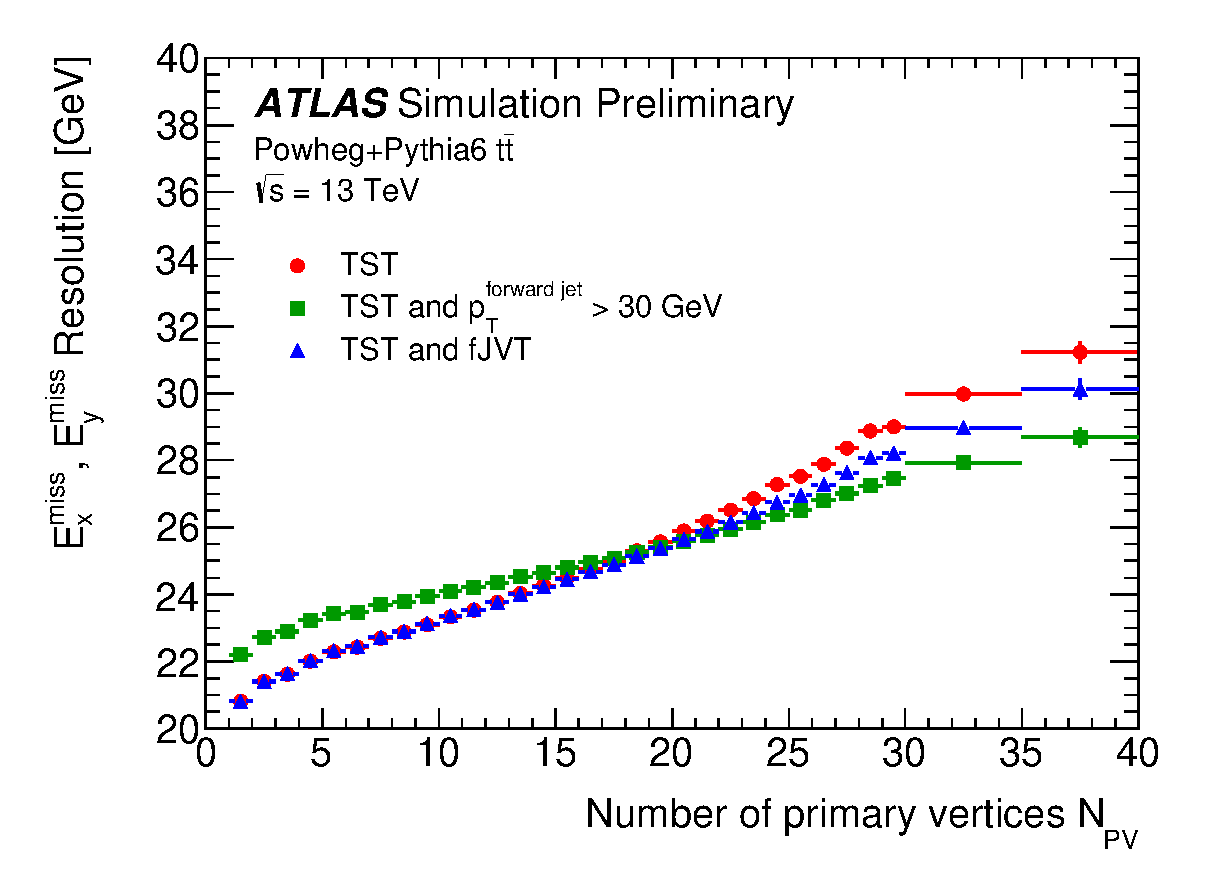
\includegraphics[width=0.48\textwidth]{figures/METCalib/MET_TST_tt.eps}
\caption{Uncertainty on the $\met$ track soft term (TST) vs the number of reconstructed vertexes.  }
\label{fig:sys:MET_TST_tt}
\end{center}
\end{figure}

\indent The $\met$ soft term resolution and scale uncertainty contribute a $1-2\%$ uncertainty on the total background yield.  The small uncertainty result from the high required $\met$ of at least 250 $\gev$ and little to no extrapolation across $\met$ between CR and SR for all major backgrounds. \\

\subsubsection*{Uncertainty on Lepton Reconstruction Efficiencies and Energy Scale}

\indent Uncertainty on lepton reconstruction and identification propagate to uncertainty on CR and SR yields.  These uncertainties include uncertainties on e/$\gamma$ resolution, energy scale, and reconstruction efficiency and muon momenta and reconstruction efficiency.  Lepton trigger scale factors are taken into account for the $\ttbar+\gamma$ control region. \\

\indent These uncertainties are derived by the ATLAS E/$\gamma$ and muon combined performance groups and result in sub 1\% uncertainty on signal region yields. \\

\subsubsection*{Pileup}

\indent The uncertainty on the amount of pileup in 2015 and 2016 ATLAS data is estimated using a two sided variation in event weights.  Pile-up uncertainty contributes a 1-2\% uncertainty on the total background yield in the SR.



  % The detector systematic uncertainties above are calculated as the variations in the shapes of the original normalized histograms using ${\tt overallNormHistoSys}$ inside ${\tt HistFitter}$.
% \item{\bf Luminosity}
%The uncertainty of 2.8 $\%$ is assigned for the integrated luminosity and is denoted by {\bf Lumi} in the fit.


  %%%%%%%%%%%%%%%%%%%%%%%%%%%%%%%%%%%%%%%%%%%%%%%%%%%%%%%%%%
  %% Commented out for the time being since the est, method are not fully defined yet
  %%%%%%%%%%%%%%%%%%%%%%%%%%%%%%%%%%%%%%%%%%%%%%%%%%%%%%%%%%
%% \item{\bf Z fit method for $Z+jets$ background}
%% Following the detailed study in Section~\ref{section:Z_Results}, the uncertainty of 17
%% $\%$ is assigned to $Z+jets$ background for the $Z+jets$ fit-method estimation and is denoted by {\bf methodSysZ} in the fit.

%% \item{\bf Jet-smearing estimation method for multi-jet background}
%% The uncertainty of 100 $\%$ to is conservatively assigned to the
%% multi-jet yields for the jet-smearing estimation method and is denoted by
%% {\bf theoSysQCD} in the fit.

%% \item{\bf \dphimettrk\ and tau veto}
%%   No additional uncertainty is assigned for the requirements on
%%   \dphimettrk\ and on the tau veto. Both were discussed extensively for
%%   the 7 \TeV\ analysis \cite{7TeVSupportNote} where no additional
%%   systematic was assigned.  There are currently no official
%%   recommendations from the jet/etmiss group for \mettrk.  For the 7
%%   \TeV\ analysis, Fig 42 in Appendix C showed good agreement between
%%   data and MC for \dphimettrk\ in the tau-veto-inverted validation
%%   region.  For the current analysis, Fig. \ref{fig:SRA_dataMC} shows
%%   good agreement for the \mettrk\ variables in a \ttbar\ dominated
%%   region.  Tau veto systematics are documented in Appendix D of the 7
%%   \TeV\ note.  Data/MC comparisons were made for several variables in
%%   the 1-lepton control region and in the tau-veto-inverted validation
%%   region.  The tau fake rate was determined in a $Z\nu\nu$+jets
%%   dominated sample to be around 12\%. The systematic on this fake rate
%%   was determined with a study of the track multiplicity in jets; the
%%   track multiplicity for ($n_{trk} \le 4$) showed agreement within 5\%
%%   between data and MC.

  %%%%%%%%%%%%%%%%%%%%%%%%%%%%%%%%%%%%%%%%%%%%%%%%%%%%%%%%%%
  %%%%%%%%%%%%%%%%%%%%%%%%%%%%%%%%%%%%%%%%%%%%%%%%%%%%%%%%%%
  

  



\subsection{Theoretical Uncertainties}
\label{sec:TheoSystematics}

\indent Theoretical uncertainties quantify the uncertainty associated with MC generation including calculations on the matrix element, parton shower, and different scale parameters such as QCD renormalization, factorization scales and $\alpha_s$ etc.  As the background is ultimately normalized to the CR, only difference comes from the transfer factor (defined in equation \ref{eqn:TF}) will result in a different SR background yield.  \\

\begin{equation}
T = \frac{N_{MC}^{SR}}{N_{MC}^{CR}}
\label{eqn:TF}
\end{equation}

\indent We vary MC generation with respect to the default setting and determine the corresponding variation in the transfer factor according to equation \ref{eq:theory_uncertainty}.  All theoretical uncertainties for different backgrounds are assumed to be independent of one another. \\

 \begin{eqnarray}
    \Delta_{X} = \frac{T_f^{\mathrm{up}} - T_f^{\mathrm{down}}}{T_f^{\mathrm{up}} + T_f^{\mathrm{down}}}
    \label{eq:theory_uncertainty}
  \end{eqnarray}

\subsubsection*{$\ttbar$ Theoretical Uncertainty}

\indent Theoretical uncertainties on ttbar production include uncertainties on the hard scattering matrix element (ME) calculation, uncertainties on the parton shower (PS), and uncertainty on the amount of ISR/FSR produced in association with ttbar.  \\

%\indent The ttbar ISR/FSR uncertainty is estimated by performing the analysis on fully reconstructed simulation with variations on the PS tuning and ME+PS matching scales that induces more/less ISR and FSR in the simulation. 

\indent  The ttbar ISR/FSR uncertainty is estimated by using the radHi and radLo $\powheg\pythia$ samples.  These samples are produced with different renormalization and factorization scales compared to the nominal sample (x0.5 to radHi and x2 to radLo).   The radHi sample also increase the $h_{damp}$ parameter that help control the matching between PS and ME from the nominal $m_{top}$ to $2 \times m_{top}$. In general, the radHi (radLo) sample generates a higher (lower) differential cross-section for ttbar that is produced in conjunction with strong ISR.  \\

%\indent The uncertainty on the ME calculation and on the PS calculation is estimated by performing the analysis on truth level-simulation using different MC generator programs.  In short, the ISR/FSR uncertainty determines how much the ttbar yields in SR differ if different $\powheg$ and $\pythia$ settings were used.  The ttbar hard scattering and PS variations determines how much the ttbar yields in SR differ if different generator programs and parton shower tunes are used. \\

\indent Uncertainties on the hard scattering and PS are calculated by comparing the nominal $\powheg\pythia$ ttbar sample with $\powheg\herwigpp$ ttbar and $\sherpa$ 2.2.1 ttbar samples.  The $\powheg\herwigpp$ sample do not vary the ME calculation with respect to the nominal sample but does perform a different set of PS calculation with a distinct PS tune.  The $\sherpa$ 2.2.1 ttbar sample perform a different ME and PS calculation with a different PDF set and PS tune.  More details on the different ttbar MC generation can be found in section \ref{sec:MC:Bkg}. \\

\indent We take an envelope of the $\sherpa$ and $\powheg\herwigpp$ variations as the combined ttbar hard scattering and PS uncertainty.  This is because the $\powheg\herwigpp$ and $\sherpa$ samples both vary the PS and avoids double counting of the PS uncertainty. The total hard scattering plus PS uncertainty is defined as the maximum of equation \ref{eq:ttbar_ME_uncertainty} and \ref{eq:ttbar_PS_uncertainty}.  \\

    \begin{eqnarray}
      \Delta_{\mathrm{hard~scatter}} = \frac{T_f^{\mathrm{\powheg}} - T_f^{\mathrm{\sherpa}}}{T_f^{\mathrm{\sherpa}}}
      \label{eq:ttbar_ME_uncertainty}
    \end{eqnarray}

    \begin{eqnarray}
      \Delta_{\mathrm{PS}} = \frac{T_f^{\mathrm{\pythia}} - T_f^{\mathrm{\herwigpp}}}{T_f^{\mathrm{\pythia}}}
      \label{eq:ttbar_PS_uncertainty}
    \end{eqnarray}
 
\indent The pre-fit $\ttbar$ yields in CR, VR and SR for the different ttbar samples and the ttbar theory uncertainty derived from transfer factor are given in table \ref{tab:ttbar_unc_SRC}  \\
  
   \begin{table}[!h]
    \begin{center} \footnotesize
      \begin{tabular}{|c|c|c|c|c|c|c|c|}
        \hline
        & $\ttbar$ CR & SRC1 & SRC2 & SRC3 & SRC4 & SRC5 & $\ttbar$ VR\\
        \hline
ttbar&   $668\pm 9 $&    $16.7\pm 1.6 $&         $31.7\pm 2.1 $&         $21.7\pm 1.6 $&         $6.3\pm 0.8 $&          $0.60\pm 0.23 $&         $232\pm 5 $\\
ttbar (rad up)&          $872\pm 11 $&   $25.2\pm 2.3 $&         $39.5\pm 2.3 $&         $28.7\pm 2.1 $&         $8.6\pm 1.0 $&  $1.05\pm 0.33 $&         $293\pm 7 $\\
ttbar (rad down)&        $521\pm 9 $&    $10.1\pm 1.0 $&         $19.2\pm 1.6 $&         $15.8\pm 1.5 $&         $6.3\pm 1.2 $&  $0.7\pm 0.4 $&   $187\pm 5 $\\
ttbar (Powheg+H++)&      $621\pm 10 $&   $16.3\pm 1.8 $&         $27.8\pm 1.8 $&         $18.0\pm 1.5 $&         $6.5\pm 0.9 $&  $0.46\pm 0.18 $&         $206\pm 5 $\\
ttbar (Sherpa)&          $840\pm 40 $&   $30\pm 8 $&     $42\pm 9 $&     $22\pm 5 $&     $7.4\pm 3.2 $&          $<0.01$&        $297\pm 30 $\\        
        \hline
        \multicolumn{8}{c}{\bf Transfer factors (in \%)} \\ \hline
        ISR/FSR &  &      $20$&   $10$&   $4$&    $10$&   $5$&    $3.3$\\
        PS &     &   $5$&    $6$&    $11$&   $11$&   $20$&   $4$\\
        hard scattering &    &    $40$&   $5$&    $19$&   $10$&   $100$&          $2$\\
        \hline       
        \end{tabular}
    \end{center}
    \caption{Expected yields for different ttbar samples and theory uncertainties based on transfer factor for the $\ttbar$ background for the SR, ttbar CR and VR.}
    \label{tab:ttbar_unc_SRC}
  \end{table}

\subsubsection*{$\Wjets$ Theoretical Uncertainty}

\indent The $\sherpa$ generator is used to estimate $\Wjets$ theory uncertainties.  Different scale variations and seven LHE3 variations are included to model the variations in $\sherpa$ parton shower and ME calculations.  \\

\indent The theory uncertainty on $\Wjets$ production obtained from transfer factors is given in table \ref{tab:WThSyst}.  Values are given as percent uncertainty on $\Wjets$ yields in the SR.  \\

  \begin{table}[!h]
    \begin{center} \footnotesize
\begin{tabular}{c||c} \hline\hline
{\bf SR} & {\bf uncertainty (\%)} \\ \hline
SRA-TT & 9.5\\ \hline
SRA-TW & 8.0\\ \hline
SRA-T0 & 6.1\\ \hline
SRB-TT & 9.1\\ \hline
SRB-TW & 7.9\\ \hline
SRB-T0 & 3.3\\ \hline
SRC1 & 11.4\\ \hline
SRC2 & 12.5\\ \hline
SRC3 & 11.8\\ \hline
SRC4 & 10.7\\ \hline
SRC5 & 9.5\\ \hline
SRC6 & 11.3\\ \hline
SRD-low & 8.8\\ \hline
SRD-high & 8.2\\ \hline
SRE & 9.5\\ \hline
VRW & 1.9\\ \hline
\hline
\end{tabular}

    \end{center}
    \caption{Summary of the theory uncertainties (in percent) on $W$ production obtained using variations on transfer factors. }
    \label{tab:WThSyst}
  \end{table}        

\subsubsection*{Single Top Theoretical Uncertainty}

\indent Single top theoretical uncertainty include uncertainty on the PS, ISR/FSR, and the interference between ttbar and single top in the Wt channel.  Single top uncertainties is evaluated on the $Wt$ subprocess because the $Wt$ subprocess dominates the single top background in signal region.  \\

\indent The single top parton shower uncertainty is modeled by comparing the nominal $\powheg\pythia$ sample with a $\powheg\herwigpp$ single top sample in a similar fashion to the ttbar PS uncertainty.  \\

\indent The single top ISR/FSR uncertainty is also modeled by comparing the radHi and radLo $\powheg\pythia$ single top samples to the nominal $\powheg\pythia$ samples analogous to the $\ttbar$ ISR/FSR uncertainty. \\

\indent The single top interference uncertainty refer to the fact that at NLO the calculation of the $pp \rightarrow Wt$ process will include contributions from $ pp \rightarrow \ttbar \rightarrow t + b + W$ which is already modeled in the SM ttbar MC.  We can subtract out the ttbar contribution at either the level of amplitude (DR scheme) or at the level of matrix elements (DS scheme).  Subtracting at the matrix element level also remove any potential interference between the single top $pp \rightarrow Wt$ and ttbar $ pp \rightarrow \ttbar \rightarrow t + b + W$ processes.  Subtracting at the amplitude level does not remove those interferences. \\

\indent  Both DR and DS schemes violates formal gauge invariance and there is no consensus on the correct procedure to treat the ttbar and single top interference.  We quantify the interference uncertainty by taking the difference between the DR and DS schemes.  \\

\indent At the moment we take an 100\% interference uncertainty because of the low MC statistics in DS scheme. \\

\indent The pre-fit single top yields in SR, single top CR and VR for the different single top samples and the single top theory uncertainty derived from transfer factor is given in table \ref{tab:single_top_unc3}. \\

   \begin{table}[!h]
    \begin{center} \footnotesize
        \begin{tabular}{|c|c|c|c|c|c|c|c|}
        \hline
        & CRST  & SRC1 & SRC2 & SRC3 & SRC4 & SRC5 & VRTopC\\ \hline
          \hline
          st Wt (MET200)&          $41.7\pm 1.1$&          $0.66\pm 0.14$&         $1.14\pm 0.18$&         $0.99\pm 0.17$&         $0.39\pm 0.11$&         $0.12\pm 0.06$&         $19.9\pm 0.8$\\
          st Wt (radHi, MET200)&   $50.4\pm 1.3$&          $0.60\pm 0.14$&         $1.26\pm 0.20$&         $1.33\pm 0.21$&         $0.57\pm 0.14$&         $0.25\pm 0.09$&         $21.9\pm 0.8$\\
st Wt (radLo, MET200)&   $34.9\pm 1.0$&          $0.57\pm 0.13$&         $0.77\pm 0.15$&         $0.77\pm 0.15$&         $0.37\pm 0.10$&         $0.09\pm 0.05$&         $16.9\pm 0.7$\\
st Wt (Powheg+H++,MET200)&       $39.2\pm 1.0$&          $0.62\pm 0.13$&         $0.84\pm 0.16$&         $0.79\pm 0.15$&         $0.38\pm 0.10$&         $0.08\pm 0.05$&         $18.7\pm 0.7$\\
st Wt (DS,MET200)&       $6.8\pm 0.4$&   $0.12\pm 0.05$&         $0.30\pm 0.09$&         $0.23\pm 0.08$&         $0.16\pm 0.06$&         $0.020\pm 0.020$&       $4.39\pm 0.31$\\
          \hline \hline 
          \multicolumn{8}{c}{\bf Transfer factors (in \%)} \\ \hline
          ISR/FSR& &       $16\pm17$&      $6\pm13$&       $9\pm13$&       $3\pm18$&       $32\pm32$&      $5.4\pm3.4$\\
          PS &   &     $0\pm30$&       $22\pm22$&      $15\pm24$&      $0\pm40$&       $30\pm70$&      $0\pm7$\\
          Interference (DR vs DS) &  &      $10\pm50$&      $60\pm50$&      $40\pm50$&      $150\pm110$&    $0\pm110$&      $35\pm13$\\
          \hline
        \end{tabular}
    \end{center}
    \caption{Summary of the single-top theory uncertainties obtained in each of the signal regions. The uncertainties are symmetrize, and all numbers are given in percentages.}
    \label{tab:single_top_unc3}
  \end{table}

\subsubsection*{$\ttV$ Theoretical Uncertainty}

\indent $\ttV$ theoretical uncertainty include scale variations and \texttt{NNPDF3.0} PDF variations.  Plus an uncertainty on the difference between $\ttbar\gamma$ and $\ttbar Z$ vector boson $\pt$ differential cross section is added for $\ttV$ due to the procedure of using $\ttbar+\gamma$ to estimate $\ttV$.  $\sherpa$+OpenLoops is used to calculate $\ttbar \gamma$ and $\ttbar Z$ vector boson differential cross-section to NLO accuracy.  The relative difference between $\sherpa$+OpenLoops and the nominal {\sc MadGraph5\_aMC\/@NLO} cross-sections is combined in quadrature with the scale and \texttt{NNPDF3.0} PDF variations to give the total $\ttV$ theoretical uncertainty. \\

\indent $\ttV$ theoretical uncertainty is given in table \ref{ab:ttbarZ_unc1}.  The systematic uncertainty maybe large for $\ttV$ production in the SR but $\ttV$ comprise about 1\% of our expected background. Therefore, $\ttV$ do not contribute significantly to the total background uncertainty in the analysis. \\

  \begin{table}[!h]
    \begin{center} \footnotesize
      \begin{tabular}{c||c} \hline\hline
{\bf SR} & {\bf uncertainty (\%)} \\ \hline
SRA-TT & 5.2\\ \hline
SRA-TW & 4.0\\ \hline
SRA-T0 & 0.8\\ \hline
SRB-TT & 3.3\\ \hline
SRB-TW & 5.0\\ \hline
SRB-T0 & 1.2\\ \hline
SRC1   & 35.3\\ \hline
SRC2   & 5.5\\ \hline
SRC3   & 6.6\\ \hline
SRC4   & 19.7\\ \hline
SRC5   & 23.7\\ \hline
SRD-low & 3.4\\ \hline
SRD-high & 6.5\\ \hline
SRE & 2.7\\ \hline
\hline
\end{tabular}

    \end{center}
    \caption{Summary of the theory uncertainties (in percent) on $\ttV$ production obtained on the transfer factor. The uncertainties are symmetries.}
    \label{tab:ttbarZ_unc1}
  \end{table}

\subsubsection*{Dibosons Theoretical Uncertainty}

A 50\% uncertainty is used for the dibosons estimate because the diboson yield is predicted using MC alone.

\subsubsection*{$Z$+jets Theoretical Uncertainty}

A 50\% uncertainty is used for the $\Zjets$ estimate because the $\Zjets$ yield is predicted using MC alone.

%\subsubsection*{Signal Theoretical Uncertainty}

%  {\color{red} Coming soon}
